\renewcommand{\lastmod}{2. Dezember 2024}
\renewcommand{\chapterauthors}{Markus Lippitz}

\chapter{Atome im Magnetfeld}






\section{Überblick}

In diesem letzten Kapitel zur Atomphysik werden wir den Einfluss des Magnetfeldes auf die Spektren der Atome diskutieren. Zuerst werde ich jedoch das \emph{Einstein-de Haas-Experiment} nachreichen, das bereits bei der Einführung des Spins erwähnt wurde. Dieses Experiment zeigt, dass der Spin der Elektronen tatsächlich mit einem Drehimpuls verbunden ist. Beim Umpolen eines Magnetfeldes wirkt auf einen magnetisierbaren Zylinder ein Drehmoment. Die Größe dieses Drehmoments zeigt, dass der Elektronenspin pro Einheit des Drehimpulses doppelt so viel magnetisches Moment erzeugt wie ein Bahndrehimpuls.

Der zentrale Effekt dieses Kapitels ist jedoch der \emph{Zeeman-Effekt}: Die Spektrallinien atomarer Übergänge spalten auf, wenn ein Atom in ein Magnetfeld gebracht wird. Die magnetischen Momente, die mit dem Spin und dem Bahndrehimpuls verknüpft sind, liefern einen Energiebeitrag, der von der Orientierung der Momente im Magnetfeld abhängt. Historisch gesehen konnte man vor der Entdeckung des Elektronenspins nur bestimmte Spektren verstehen. Dies wurde als 'normaler' Zeeman-Effekt bezeichnet. Er liefert immer drei Linien. Der 'anomale' Zeeman-Effekt liefert ein komplizierteres Spektrum, da die relative Orientierung von Spin und Bahndrehimpuls einen zusätzlichen Freiheitsgrad liefert. Diese führt auch zum \emph{Landé g-Faktor}, der eine Art effektives magnetisches Moment beschreibt.

Dieses Kapitel folgt \cite{Harris_moderne_Physik} mit großen Anteilen von \cite{Demtröder_ep3}.





\section{Drehimpuls und magnetisches Moment}

Bei der Einführung des Spins hatten wir bereits kurz den Zusammenhang mit dem magnetischen Moment erwähnt. Auf dieses wirkt schließlich die Kraft im Stern-Gerlach-Experiment. Die genauere Diskussion wird hier nachgeholt.

Stellen wir uns zunächst ein Elektron auf einer klassischen Kreisbahn vor. Die Kreisbahn entspricht einem Strom $I$ und definiert auch eine Fläche $A$. Durch die Flächennormale können wir auch einen Vektor $\bA$ definieren, dessen Betrag der Fläche und dessen Richtung der Flächennormalen entspricht. Damit ist das magnetische Dipolmoment $\bmu$ der klassischen Elektrodynamik 
\begin{equation}
    \bmu = I \bA = \frac{-e}{T} \, \pi r^2 = - \frac{e}{2\pi r/v} \, \pi r^2 
%= -\frac{e}{2} \, vr 
= -\frac{e}{2m} \, m v r = - \frac{e}{2m} \bl
\end{equation}
wobei in den Zwischenschritten die Richtung des Vektors weggelassen wurde. Ein klassischer Drehimpuls aufgrund einer Bahnbewegung ist also mit einem magnetischen Dipolmoment verbunden. Die Proportionalitätskonstante zwischen dem magnetischen Moment und dem Drehimpuls wird \emph{gyromagnetisches Verhältnis} $\gamma$ genannt
\begin{equation}
    \gamma  = \frac{|\bmu|}{|\bl|} = g \, \frac{e}{2m} = g \frac{\mu_B}{\hbar} \quad .
\end{equation}
Dabei haben wir schon mal den Landé-g-Faktor eingeführt, der hier für den Bahndrehimpuls natürlich $g=1$ ist, und das \emph{Bohr'sche Magenton} 
\begin{equation}
\mu_B = \frac{e \hbar}{2 m_e} = 9.27 \cdot 10^{-24} \text{ J/T}     \quad .
\end{equation}



In einem äußeren Magnetfeld $\bB$ führt ein Drehimpuls eine Präzessionsbewegung aus. Es wirkt ein Drehimpuls $\btau = \bmu \times \bB$, der immer senkrecht zum Dipolmoment $\bmu$ und damit auch senkrecht zum Drehimpuls $\bl$ steht. Das ist genau wie bei einem Kreisel im Gravitationsfeld der Erde. Die Spitze des Drehimpulsvektors beschreibt also eine Kreisbahn senkrecht zu $\bB$:
\begin{equation}
    \frac{d \bl}{dt} = - \frac{e}{2m} \, \bL \times \bB  \quad .
\end{equation}
Die Frequenz der Kreisbewegung nennt man \emph{Lamor-Frequenz}\sidenote{nach Joseph Larmor, irischer Physiker und Mathematiker, 1857--1942}
\begin{equation}
    \omega_\text{Lamor} = \gamma | \bB |  \quad .
\end{equation}


\section{Einstein-de Haas-Experiment}


Bei der Einführung des Elektronenspins habe ich bisher nur behauptet, dass dieser auch mit einem Drehimpuls verbunden ist. Das Einstein-de Haas-Experiment beweist, dass der Drehimpuls des Elektronenspins tatsächlich existiert.

\begin{marginfigure}
    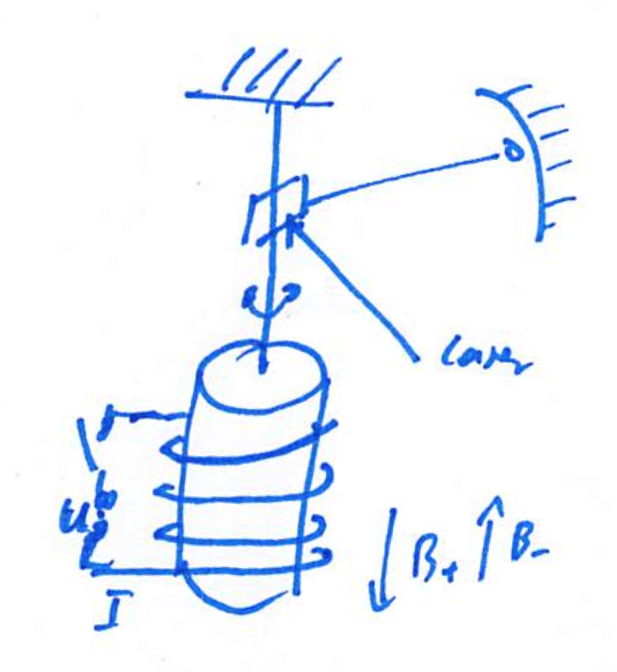
\includegraphics[width=\textwidth]{\currfiledir png/einstein-de-haas.png}
    \caption{Einstein-de Haas-Experiment}
\end{marginfigure}

Ein Eisenzylinder bekannter Größe und Masse ($m$, $R$, $V$) ist an einem Torsionspendel der Federkonstante $k$ aufgehängt. Der Zylinder hängt in einer Spule, mit der ein äußeres Magnetfeld (anti)parallel zum Zylinder erzeugt werden kann. Zunächst wird die statische Sättigungsmagnetisierung $M_+$ und $M_-$ für beide Feldrichtungen gemessen. In der dynamischen Messung wird das Drehmoment aus der Umkehrung der Drehimpulse gemessen. Der Zylinder dreht sich und ein Lichtzeiger ermöglicht die Bestimmung der maximalen Auslenkung $\phi$. In der Praxis ist der Effekt so klein, dass $\phi$ nicht direkt gemessen werden kann, sondern eine getriebene Oszillation auf der Resonanz des Pendels verwendet wird. Dies wird hier vernachlässigt. 

Durch die Umkehrung des Magenfeldes ändert sich die z-Komponente des Drehimpulses von $l_z$ zu $-l_z$. Die Änderung des Zylinder-Drehimpulses ist also 
\begin{equation}
    \Delta L = 2 N l_z
\end{equation}
mit der Anzahl $N$ der Atome im Zylinder. Aus der Energieerhaltung (Federpotential gleich kinetische Energie in der Drehbewegung) ergibt sich eine Beziehung zwischen $\phi$ und $\Delta L$.
\begin{equation}
\frac{\Delta L ^2}{2 (mR^2/2)} = \frac{k \phi^2}{2}    \quad .  
\end{equation}
Die Änderung des magnetischen  Moments des Zylinder $\mu_\text{Zyl}$ ist
\begin{equation}
   \Delta  \mu_\text{Zyl} = V | M_+ - M_-| = 2 N \mu_z
\end{equation}
mit $\mu_z$ der z-Komponente des atomaren magnetischen Moments. Das gyromagnetische Verhältnis ist
\begin{equation}
    \frac{ \Delta  \mu_\text{Zyl}}{\Delta L}
    = \frac{|\mu_z|}{|l_z|} = \gamma = g \frac{\mu_B}{\hbar}  \quad .
\end{equation}
Das Einstein-de Haas-Experiment bestimmt also den Landé g-Faktor. Bei Eisen tragen die Bahndrehimpulse der Elektronen nur wenig zum Magnetismus bei, da die 6 Valenz-Elektronen in der  3d-Schale beinahe alle 7 $m_l$-Werte besetzen. 
Der Magnetismus wird hauptsächlich durch die Elektronenspins verursacht. Die Bewegung des Zylinders demonstriert also, dass der Elektronenspin tatsächlich mit einem Drehimpuls verbunden ist! 

Im Experiment findet man $g \approx 2$, also doppelt so groß wie beim Bahndrehimpuls. Klassischerweise hätte man $g=1$ wie für den Bahndrehimpuls erwartet. Die relativistische Erweiterung der Quantenmechanik (Dirac-Gleichung) liefert $g=2$. Erst die Quantenelektrodynamik liefert $g=2,002319\dots$. Dieser Wert ist mit 13 Nachkommastellen extrem genau bekannt und stimmt mit der Theorie überein.


\section{Normaler Zeeman-Effekt}

Bei den quantenmechanischen Drehimpulsen hatten wir immer eine ausgezeichnete Richtung definiert, die z-Richtung, entlang der die Komponente $m_L$ des Drehimpulses $\bL$ zusammen mit seiner Länge $L$ angegeben werden kann. Diese Richtung war bisher beliebig. Wenn ein äußeres Magnetfeld angelegt wird, dann definiert dieses Magnetfeld die Richtung. Um mit unseren Bezeichnungen konsistent zu bleiben, legen wir das Magnetfeld immer in z-Richtung an. Die Energie der magnetischen Momente in diesem Magnetfeld ist dann ein zusätzlicher Beitrag in der Energiehierarchie. Wir diskutieren zunächst den einfachen Grenzfall, dass diese Energie viel kleiner ist als alle anderen Energien, also kleiner als die Coulomb-Abstoßung  der Elektronen und kleiner als die der Spin-Bahn-Kopplung. Danach betrachten wir kurz den anderen Extremfall.

Die Energie eines magnetischen Moments $\bmu$ im Magnetfeld $\bB$ ist $E = - \bmu \cdot \bB$. Da ein Drehimpuls in der Quantenmechanik nur diskrete Orientierungen relativ zur Vorzugsrichtung einnehmen kann, gilt dies auch für das magnetische Moment. Dies führt dazu, dass alle Zustände entsprechend der Orientierungsmöglichkeiten weiter aufspalten. Dieser Einfluss des Magnetfeldes wird als \emph{Zeeman-Effekt} bezeichnet. 

Wir beginnen mit dem 'normalen' Zeeman-Effekt. Aus heutiger Sicht ist das eher ein Spezialfall. Historisch gesehen war er aber derjenige, den man gut verstehen konnte. Hier spielt der Spin der Elektronen keine Rolle. Dies ist immer dann der Fall, wenn der atomare Zustand die Quantenzahl $S=0$ hat. Wie wir wissen, kommt das manchmal vor, aber es ist nicht der Normalfall.

Sei also $S=0$. Damit ist das magentische Moment nur noch durch $L$ gegeben und $\bmu = - \bL \mu_B / \hbar$ bzw. $\mu_z = - \mu_B  m_L$. Die Energieänderung $\Delta E$ ist
\begin{equation}
    \Delta E = - \bmu \cdot \bB =- \mu_z B =  \mu_B \, m_L \, B  \quad .
\end{equation}
Jeder Zustand spaltet also in $2L + 1$ Niveaus auf, die voneinander dem Abstand $\mu_B B$ haben.

Hier kommt die Auswahlregel $\Delta m_J = 0, \pm1$ aus dem letzten Kapitel zum Tragen. Es gibt zwei Möglichkeiten: Alle anderen Quantenzahlen können gleich bleiben und es gibt nur einen Übergang $\Delta m_J = \pm1$ zum nächsten benachbarten Zeeman-Niveau. Dazu benötigt man eine elektromagnetische Welle mit der Frequenz $\hbar \omega = \mu_B B$. Bei einem Feld von $B=1$~mT entspricht dies einer Frequenz von etwa 10~MHz. Dies ist die Grundlage aller Spinresonanztechniken, wie der Kernspinresonanz (NMR) und verwandter bildgebender Verfahren (MRI). Die zweite Möglichkeit ist, dass sich auch andere Quantenzahlen ändern. Dies sind dann optische Übergänge, die spektral um eben diese ca. 10~MHz aufspalten. Die Anzahl der Linien ergibt sich aus den möglichen Werten von $m_J$ in den beiden beteiligten Zuständen und den Auswahlregeln.


In beiden Fällen spielt auch der Zusammenhang zwischen $\Delta m_J = 0, \pm1$ und der Polarisation des Photons eine Rolle, wie wir im letzten Kapitel gesehen haben. Die Übergänge zeigen in der Emission bzw. erfordern in der Absorption eine entsprechende zirkulare oder lineare Polarisation.


\paragraph{Nebenbemerkung} Die Feinstrukturaufspaltung aufgrund der Spin-Bahn-Kopplung kann als (normaler) Zeeman-Effekt des Elektronenspins im Magnetfeld des Kerns verstanden werden. Dies führt zum gleichen Ergebnis.

\section{Beispiel: Cadmium}

Cadmium hat die Elektronenkonfiguration [Kr]4d$^{10}$ 5s$^2$. Dies ist ein $^1S_0$-Zustand. Wir betrachten hier den Übergang ($\lambda \approx 643.8$~nm) zwischen den beiden angeregten Zuständen $^1D_2$ und $^1P1$. Dabei ändert sich nur die Wellenfunktion des Leuchtelektrons von 5d nach 5p. Alle beteiligten Zustände sind Singulett-Zustände mit $S=0$, der Spin spielt keine Rolle und es tritt der Normale Zeeman-Effekt auf. Beide Zustände spalten sich im Magnetfeld in $2J+1$ Zeeman-Niveaus auf, also in 5 bzw. 3 Niveaus. Alle Abstände sind gleich $\Delta E = \mu_B B$. Aufgrund der Auswahlregel $\Delta m_J = 0, \pm1$ gibt es im Spektrum nur drei Linien mit jeweils gleichem $\Delta m_J$.

\begin{marginfigure} 
    \inputtikz{\currfiledir cadmium_Bfeld}
    \caption{Normaler Zeeman-Effekt in \ch{Cd}.}
\end{marginfigure}


\section{Anomaler Zeeman-Effekt}

Nun kommen wir zum 'anomalen' Zeeman-Effekt. Bevor der Elektronenspin entdeckt und verstanden wurde, waren die Spektren vieler Atome im Magnetfeld unverständlich. Die Anzahl der Linien war nicht gleich drei, wie man es beim normalen Zeeman-Effekt erwarten würde. Deshalb nannte man das damals 'anomal'. Aus heutiger Sicht ist das nicht mehr ungewöhnlich, sondern nur noch eine kleine Rechenhürde.

Wenn also $S \neq 0$ ist, dann ist die Beziehung zwischen Drehimpuls und magnetischem Moment relevant:
\begin{equation}
    \bmu_L = - g_l \frac{\mu_B}{\hbar} \, \bL \quad \text{und} \quad  \bmu_S = - g_s \frac{\mu_B}{\hbar} \, \bS
\end{equation}
mit $g_l = 1$ und $g_s \approx 2$. Das gesamte Magnetische Moment ist die Summe
\begin{equation}
    \bmu_J =  \bmu_L +  \bmu_S = - \frac{\mu_B}{\hbar} \left( \bL + g_s \bS \right)  \quad .
\end{equation}
Wenn $g_s = g_l$ wäre, dann wäre $\bmu_J$ proportional zu $\bJ$ und insbesondere genau entgegengesetzt zu $\bJ$. Dies ist nicht der Fall, und dies ist der Grund für die folgende Rechnung.

Nehmen wir zunächst an, dass es kein äußeres Magnetfeld $\bB$ gibt. Dann sind die Längen $S$, $L$ und $J$ zeitlich konstant und die z-Komponente  $m_J$, nicht aber $m_S$ und $m_L$. Das bedeutet, dass die Spitze von $\bS$ eine Kreisbahn in einer Ebene senkrecht zu $\bJ$ beschreibt. Da das magnetische Moment die oben genannte Summe aus $\bS$ und $\bL$ enthält, beschreibt die Spitze von $\bmu_J$ ebenfalls eine Kreisbahn um die durch $\bJ$ definierte Achse.

\begin{marginfigure}
    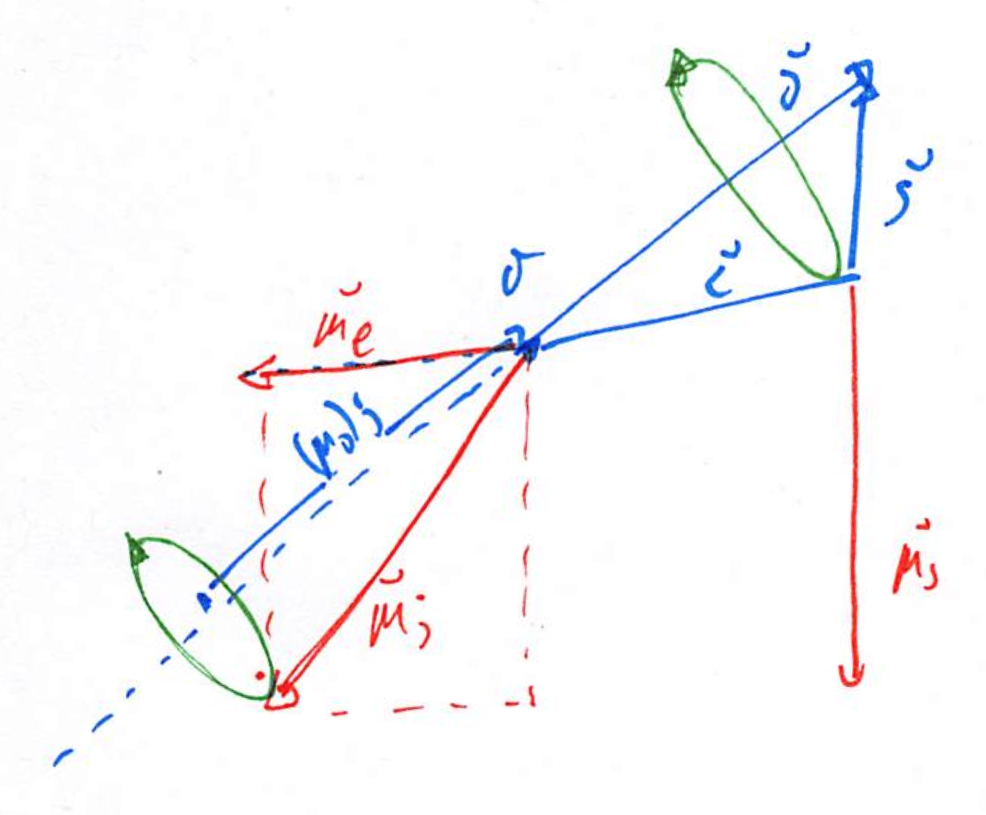
\includegraphics[width=\textwidth]{\currfiledir png/mu_average}
\caption{Der Vektor $\bmu_j$ präzediert um $\bJ$, weil $m_s$ und $m_J$ keine guten Quantenzahlen mehr sind und $g_l \neq g_s$. }
\end{marginfigure}

Relevant ist dann nur der Mittelwert von  $\bmu_J $ projiziert auf die durch $\bJ$ definierte Achse.  Diese Länge nennen wir $(\bmu_J)_J$ und berechnen sie wie folgt
\begin{equation}
    (\bmu_J)_J = \frac{\bmu_J \cdot \bJ}{|\bJ|}
    = - \frac{\mu_B}{\hbar} \left(
        \frac{\bL \cdot \bJ}{|\bJ|}
        +  g_s \,\frac{\bS \cdot \bJ}{|\bJ|}
    \right)  \quad .
\end{equation}
Wie bei der Spin-Bahn-Kopplung stellen wir Terme der Form $\bS \cdot \bJ$ bzw. $\bL \cdot \bJ$  dar, z.B.
\begin{equation}
    \bL \cdot \bJ = \frac{\hbar^2}{2}
    \left[
  J (J+1) + L(L+1 - S(S+1))
    \right]  \quad .
\end{equation}
Wenn wir diesen Term und den äquivalenten für  $\bS \cdot \bJ$  oben einsetzen, dann erhalten wir (mit $g_s = 2$)
\begin{align}
    (\bmu_J)_J = & - \mu_B \frac{3 J (J+1)+ S(S+1) - L(L+1)}{2 \sqrt{J (J+1)}} \\
    = & - g_J \frac{\mu_B}{\hbar} \, |\bj|
\end{align}
mit dem Landé-g-Faktor $g_J$ 
\begin{equation}
    g_J = 1 + \frac{J (J+1)+ S(S+1) - L(L+1)}{2 J (J+1)}   \quad .
\end{equation}
Dieser etwas merkwürdige Landé g-Faktor $g_J$ erspart uns also von nun an die Mittelung über das präzedierende magnetische Moment $\bmu_J$. Je nach relativer Länge von $\bS$, $\bL$ und $\bJ$ ist also der Zusammenhang zwischen Drehimpuls $\bJ$ und magnetischem Moment $\bmu_J$ unterschiedlich und wird durch diesen g-Faktor beschrieben. Er enthält natürlich auch die Sonderfälle, z.B. wenn $S=0$ ist, dann ist $g_J = g_l = 1$.





Nun nehmen wir das äußere Magnetfeld $\bB$ hinzu. Wir nehmen an, dass es schwächer ist als das Magnetfeld des Kerns, das zur Spin-Bahn-Kopplung führt. Die Energie der magnetischen Momente im äußeren Feld $\bB$ ist daher die niedrigste in der Energiehierarchie. Daher koppeln zunächst alle Spins zu $\bS$ und alle Bahndrehimpulse zu $\bL$. Dann richten sich die Spins im Magnetfeld des Kerns aus und die Situation wird durch einen Gesamtdrehimpuls $\bJ$ beschrieben. Das mit $\bJ$ verbundene magnetische Moment orientiert sich schließlich im äußeren Magnetfeld $\bB$. Dadurch spalten sich die Zustände  auf
\begin{equation}
    \Delta E = - \bmu_J \cdot \bB =-  (\bmu_J)_z  \, \, B =  \mu_B \, m_J \, g_J \, B  \quad .
\end{equation}
Jeder Zustand spaltet sich also in $2J+1$ äquidistante Zeeman-Niveaus auf. Da der Landé g-Faktor $g_J$ von den Quantenzahlen $S$, $L$ und $J$ abhängt, variiert er zwischen den Zuständen. Verschiedene Zustände spalten also unterschiedlich stark auf. Das ist der entscheidende Unterschied zum normalen Zeeman-Effekt. Die Folge ist, dass nicht mehr alle Übergänge mit gleichem $\Delta m_J$ bei gleicher Energie liegen. Sehr oft gibt es mehr als 3 Zeeman-Linien. 

\section{Beispiel: Natrium}

Abbildung \ref{fig:8_natrium_Bfeld} zeigt die Zeeman-Aufspaltungen der beiden Natrium-D-Linien. Der gemeinsame Grundzustand $^2S_{1/2}$ hat $g_J = 2$ und spaltet in zwei Linien auf, die bei $\pm m_J g_J = \pm 1$ mal $\mu_B B$ liegen. Die D1-Linie kommt von $^2P_{1/2}$ mit $g_J = 2/3$. Auch dieser Zustand spaltet in zwei Zustände, aber $m_J  g_J$ ist jetzt $\pm 1/3$, viel kleiner. Insgesamt gibt es 4 Linien, weil alle Kombinationen erlaubt sind.


Die D2-Linie stammt aus dem Zustand $^2P_{3/2}$ mit $g_J = 4/3$. Der Zustand spaltet in 4 Niveaus auf, die voneinander $4/3$ mal $\mu_B B$ entfernt sind. Die $\Delta m_J$ Auswahlregel verbietet den beiden extremen Zuständen $m_J = \pm 3/2$ einen Übergang zum 'gegenüberliegenden' $m_J = \mp 1/2$ des Grundzustandes, so dass es insgesamt nur $2 \times 3 = 6$ Linien gibt.


\begin{figure}
    \inputtikz{\currfiledir natrium_Bfeld}
    \caption{Anomaler Zeemaneffekt der beiden Natrium-D-Linien. Der Abstand der Ausgangszustände ist nicht maßstabsgerecht. Ebenso ändert sich die Skalierung der beiden skizzierten Spektren.}
    \label{fig:8_natrium_Bfeld}
\end{figure}


\section{Paschen-Back-Effekt}

So wie die JJ-Kopplung das Gegenteil der LS-Kopplung ist, ist der Baschen-Back-Effekt das Gegenteil des Zeeman-Effekts. Es geht immer um die Hierarchie der Energien. Bei der LS-Kopplung ist der Spin-Bahn-Beitrag am kleinsten, bei der JJ-Kopplung am größten. Für den Zeeman-Effekt haben wir angenommen, dass die Energie des mit dem Gesamtdrehimpuls verbundenen magnetischen Momentes im äußeren Magnetfeld kleiner ist als alle anderen Energien, so dass die Spin-Bahn-Kopplung unberührt bleibt. Bei wirklich sehr hohen Magnetfeldern ist aber bereits die Energie eines einzelnen Elektronenspins\sidenote{bzw. des zugehörigen magnetischen Momentes} und eines einzelnen Bahndrehimpulses im äußeren Magnetfeld höher als alle anderen Energien. Dann ist $ \bmu_s \cdot \bB$ bzw. $ \bmu_l \cdot \bB$ der dominierende Beitrag. Die Einzelspins präzedieren im Magnetfeld, die Kopplung spielt keine Rolle. Die Zustände sind also bei 
\begin{equation}
    \Delta E = \left( g_l m_l + g_s m_s \right) \, \mu_B \, B 
\end{equation}
mit $g_l = 1$ und $g_s \approx 2$. Hier sind also $m_s$ und $m_l$ 'gute' Quantenzahlen und $J$, $m_J$ spielen keine Rolle mehr, weil die Kopplungsenergie zu klein ist.

% da sollte doch ein B drin sein, oder nicht ...
% aus engl. Wikipedia
%
% Weil es die relativistischen Korrekturen aber immer noch gibt, verbleibt ein Teil der 'alten' Feinstrukturaufspaltung, so dass man insgesamt findet
% \begin{equation}
%      E = E_{n} + \frac{m_e c^2 \alpha^4}{2 n^3} 
%      \left\{ \frac{3}{4n} - \left[ \frac{l(l+1) - m_l m_s}{l(l+1/2)(l+1) } \right] \right\}
% \end{equation}


% \section{Spin-Resonanz}

% Harris 8.1.5 und 11.4

%\newpage

\section{Zusammenfassung}


\textit{Schreiben Sie hier ihre persönliche Zusammenfassung des Kapitels auf. Konzentrieren Sie sich auf die wichtigsten Aspekte.}

\vspace*{10cm}

%--------------------
\printbibliography[segment=\therefsegment,heading=subbibliography]
